\documentclass{ctexart}
\usepackage[T1]{fontenc}
\usepackage[a4paper,top=1.5cm,bottom=1.5cm,left=2cm,right=2cm,marginparwidth=1.75cm]{geometry}
\usepackage{mathtools}
\usepackage{tikz}
\usepackage{booktabs}
\usepackage{caption}
\usepackage{outlines}
\usepackage{graphicx}
\usepackage{amsthm}
\usepackage[colorlinks=false, allcolors=blue]{hyperref}
\renewcommand{\tableautorefname}{表}
\DeclarePairedDelimiter{\set}{\{}{\}}
\DeclarePairedDelimiter{\paren}{(}{)}
\graphicspath{ {./images/} }

\title{形式语言第二次作业}
\author{卢雨轩 19071125}
% \date{\today}
\ctexset{
    section = {
        titleformat = \raggedright,
        name = {,},
        number = \chinese{section}、
    },
    paragraph = {
        runin = false
    },
    today = small,
    figurename = 图,
    contentsname = 目录,
    tablename = 表,
}

\begin{document}

\maketitle

习题:p103 2.4, 2.11; p104 7, 10.6

\begin{outline}[enumerate]
    \1[2.] 构造识别下列语言的DFA(给出相应DFA的形式描述或者画出他们的
    状态转移图)。
        \2 [(4)] $\set*{x | x \in \set*{0, 1}^+ \text{ 
            且x中不含形如00的字串
        }}$

        \begin{center}
            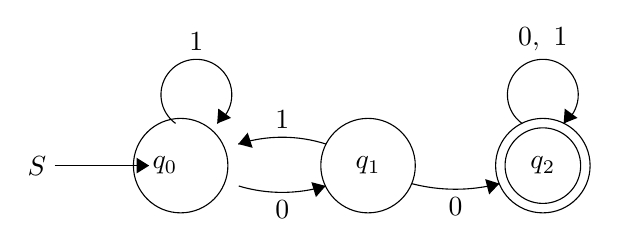
\begin{tikzpicture}[scale=0.2]
            \tikzstyle{every node}+=[inner sep=0pt]
            \draw [black] (21.9,-21.9) circle (3);
            \draw (20.9,-21.9) node {$q_0$};
            \draw [black] (33.8,-21.9) circle (3);
            \draw (33.8,-21.9) node {$q_1$};
            \draw [black] (44.9,-21.9) circle (3);
            \draw (44.9,-21.9) node {$q_2$};
            \draw [black] (44.9,-21.9) circle (2.4);
            \draw [black] (13.9,-21.9) -- (19.9,-21.9);
            \draw (13.4,-21.9) node [left] {$S$};
            \fill [black] (19.9,-21.9) -- (19.1,-21.4) -- (19.1,-22.4);
            \draw [black] (21.577,-19.22) arc (234:-54:2.25);
            \draw (22.9,-14.65) node [above] {$1$};
            \fill [black] (24.22,-19.22) -- (25.1,-18.87) -- (24.29,-18.28);
            \draw [black] (31.107,-23.195) arc (-73.28148:-106.71852:9.585);
            \fill [black] (31.11,-23.19) -- (30.2,-22.95) -- (30.49,-23.9);
            \draw (28.35,-24.1) node [below] {$0$};
            \draw [black] (25.556,-20.534) arc (107.80503:72.19497:9.137);
            \fill [black] (25.56,-20.53) -- (26.47,-20.77) -- (26.16,-19.81);
            \draw (28.35,-19.6) node [above] {$1$};
            \draw [black] (42.136,-23.042) arc (-75.35212:-104.64788:11.017);
            \fill [black] (42.14,-23.04) -- (41.24,-22.76) -- (41.49,-23.73);
            \draw (39.35,-23.9) node [below] {$0$};
            \draw [black] (43.577,-19.22) arc (234:-54:2.25);
            \draw (44.9,-14.65) node [above] {$0,\mbox{ }1$};
            \fill [black] (46.22,-19.22) -- (47.1,-18.87) -- (46.29,-18.28);
            \end{tikzpicture}
            \end{center}
        \2[(11)] $\set*{x | x \in \set*{0, 1}^+ \text{ 
            且如果x以1结尾,则他的长度是偶数;如果x以0结尾,则他的长度为奇数
        }}$
        
    \begin{center}
        \begin{tikzpicture}[scale=0.2]
        \tikzstyle{every node}+=[inner sep=0pt]
        \draw [black] (24,-10.8) circle (3);
        \draw (24,-10.8) node {偶0};
        \draw [black] (50.8,-10.8) circle (3);
        \draw (50.8,-10.8) node {奇0};
        \draw [black] (50.8,-10.8) circle (2.4);
        \draw [black] (50.8,-31.5) circle (3);
        \draw (50.8,-31.5) node {偶1};
        \draw [black] (50.8,-31.5) circle (2.4);
        \draw [black] (24,-31.5) circle (3);
        \draw (24,-31.5) node {奇1};
        \draw [black] (37.4,-21.3) circle (3);
        \draw (37.4,-21.3) node {$\epsilon$};
        \draw [black] (31,-16.7) -- (34.96,-19.55);
        \draw (30.41,-15.32) node [left] {$S$};
        \fill [black] (34.96,-19.55) -- (34.61,-18.68) -- (34.02,-19.49);
        \draw [black] (26.895,-10.014) arc (103.30426:76.69574:45.651);
        \fill [black] (47.91,-10.01) -- (47.24,-9.34) -- (47.01,-10.32);
        \draw (37.4,-8.29) node [above] {$0$};
        \draw [black] (25.056,-13.606) arc (17.24582:-17.24582:25.446);
        \fill [black] (25.06,-28.69) -- (25.77,-28.08) -- (24.82,-27.78);
        \draw (26.7,-21.15) node [right] {$1$};
        \draw [black] (47.926,-11.657) arc (-75.44172:-104.55828:41.875);
        \fill [black] (26.87,-11.66) -- (27.52,-12.34) -- (27.77,-11.37);
        \draw (37.4,-13.5) node [below] {$0$};
        \draw [black] (51.962,-13.563) arc (19.10726:-19.10726:23.177);
        \fill [black] (51.96,-28.74) -- (52.7,-28.14) -- (51.75,-27.82);
        \draw (53.74,-21.15) node [right] {$1$};
        \draw [black] (49.689,-28.715) arc (-161.799:-198.201:24.221);
        \fill [black] (49.69,-13.58) -- (48.96,-14.19) -- (49.91,-14.5);
        \draw (47.98,-21.15) node [left] {$0$};
        \draw [black] (47.859,-32.092) arc (-80.03528:-99.96472:60.444);
        \fill [black] (26.94,-32.09) -- (27.64,-32.72) -- (27.82,-31.74);
        \draw (37.4,-33.5) node [below] {$1$};
        \draw [black] (26.906,-30.755) arc (102.59162:77.40838:48.139);
        \fill [black] (47.89,-30.76) -- (47.22,-30.09) -- (47,-31.07);
        \draw (37.4,-29.1) node [above] {$1$};
        \draw [black] (22.854,-28.73) arc (-161.18818:-198.81182:23.505);
        \fill [black] (22.85,-13.57) -- (22.12,-14.17) -- (23.07,-14.49);
        \draw (21.1,-21.15) node [left] {$0$};
        \draw [black] (35.01,-23.12) -- (26.39,-29.68);
        \fill [black] (26.39,-29.68) -- (27.33,-29.6) -- (26.72,-28.8);
        \draw (29.73,-25.9) node [above] {$1$};
        \draw [black] (39.76,-19.45) -- (48.44,-12.65);
        \fill [black] (48.44,-12.65) -- (47.5,-12.75) -- (48.12,-13.54);
        \draw (45.07,-16.55) node [below] {$0$};
        \end{tikzpicture}
    \end{center}
    \1[7.] 设DFA $M=(Q, \Sigma, \delta, q_0, F)$。证明:对于
    $\forall x,y \in \Sigma^*, q \in Q, \delta(q, xy) = \delta(
        \delta(q, x), y
    )$
\begin{proof}
    不妨设$x = w_0 w_1 w_2 \dots w_n$。

    根据定义,我们有:
    \begin{align*}
        \delta(q, xy) & = \delta(q, w_0 w_1 w_2 \dots w_ny) \\
        & = \delta(\delta(q, w_0),  w_1 w_2 \dots w_ny) \\
        & = \delta(\delta(\delta(\dots \delta(q, w_n) \dots, w_1), w_0), y) \\
        & = \delta(\delta(q, w_0 w_1 w_2 \dots w_n), y) \\
        & = \delta(\delta(q, x), y) \qedhere
    \end{align*}
\end{proof}
    \1[10.] 构造识别下列语言的NFA
        \2[(6)] $\set*{x | x \in \set*{0, 1}^+ \text{
            且x中至少有两个1
        }}$
            
\begin{center}
    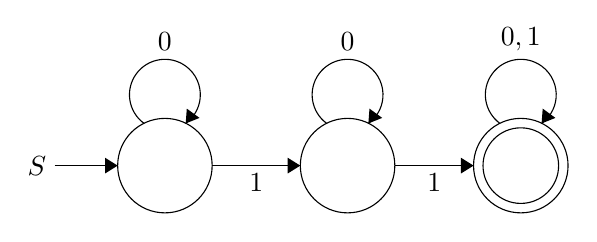
\begin{tikzpicture}[scale=0.2]
    \tikzstyle{every node}+=[inner sep=0pt]
    \draw [black] (16.8,-29.4) circle (3);
    \draw [black] (28.4,-29.4) circle (3);
    \draw [black] (39.4,-29.4) circle (3);
    \draw [black] (39.4,-29.4) circle (2.4);
    \draw [black] (19.8,-29.4) -- (25.4,-29.4);
    \fill [black] (25.4,-29.4) -- (24.6,-28.9) -- (24.6,-29.9);
    \draw (22.6,-29.9) node [below] {$1$};
    \draw [black] (31.4,-29.4) -- (36.4,-29.4);
    \fill [black] (36.4,-29.4) -- (35.6,-28.9) -- (35.6,-29.9);
    \draw (33.9,-29.9) node [below] {$1$};
    \draw [black] (27.077,-26.72) arc (234:-54:2.25);
    \draw (28.4,-22.15) node [above] {$0$};
    \fill [black] (29.72,-26.72) -- (30.6,-26.37) -- (29.79,-25.78);
    \draw [black] (15.477,-26.72) arc (234:-54:2.25);
    \draw (16.8,-22.15) node [above] {$0$};
    \fill [black] (18.12,-26.72) -- (19,-26.37) -- (18.19,-25.78);
    \draw [black] (9.8,-29.4) -- (13.8,-29.4);
    \draw (9.3,-29.4) node [left] {$S$};
    \fill [black] (13.8,-29.4) -- (13,-28.9) -- (13,-29.9);
    \draw [black] (38.077,-26.72) arc (234:-54:2.25);
    \draw (39.4,-22.15) node [above] {$0,1$};
    \fill [black] (40.72,-26.72) -- (41.6,-26.37) -- (40.79,-25.78);
    \end{tikzpicture}
    \end{center}
\end{outline}


\end{document}
